\documentclass{article}
\usepackage[T1]{fontenc}
\usepackage{iclr2027_conference,times}
\usepackage{microtype}
\usepackage{graphicx}
\usepackage{subcaption}
\usepackage{booktabs}
\usepackage{multirow}
\usepackage{amsmath}
\usepackage{amssymb}
\usepackage{mathtools}
\usepackage{xcolor}
\definecolor{linkcol}{RGB}{0,45,110}
\usepackage[colorlinks=true,allcolors=linkcol]{hyperref}
\usepackage{url}
\usepackage[capitalize,noabbrev]{cleveref}
% DRAFT MARKUP. \mock{...}: placeholder, NOT a measurement (orange). \todo{...}: missing piece (red, bracketed).
% \prelim{...}: measured from a single generation or still running; may change.
\definecolor{mockcol}{RGB}{200,90,0}
\newcommand{\mock}[1]{\textcolor{mockcol}{#1}}
\newcommand{\todo}[1]{\textcolor{red}{[TODO: #1]}}
\newcommand{\prelim}[1]{#1}
\newcommand{\method}{\textsc{Ledger+Compile}}
\renewcommand{\iclrruler}[1]{}

\title{Organize at Read Time: Query-Time Evidence Compilation\\ over an Append-Only Ledger for Long-Term Conversational Memory}
\author{Anonymous authors\\ Paper under double-blind review}

\begin{document}
\maketitle
\begin{abstract}
Most memory systems for chat assistants organize what they store as the conversation unfolds, merging and summarizing
facts before any question is asked. Whether this organization helps is unclear, because published scores confound the memory with the reader model, the answer prompt, the context budget, and the judge. We hold
these fixed on BEAM, whose conversations reach a million tokens, and find that the answer prompt and the context
budget alone open gaps as large as those between systems. We then test the alternative: \method{} stores atomic
records once and never rewrites them, and organizes them only after the question arrives, compiling retrieved records
into notes on time order, changes, conflicts, missing coverage, and the user's standing instructions. With gpt-6-luna
as the reader, it beats Hindsight, a strong write-time system given the same extra call, by \prelim{7.3} and \prelim{4.2} points on the 100K and 1M tiers (mean of three runs) while using fewer read-time tokens in total; with three stronger readers it is ahead by 1--3
points in every case, resolved in one. The lesson is to store what was said and organize it for the question; in our experiments, the benefit shrinks as the reader gets stronger. All results are on development sets, and gpt-6-luna serves as reader, memory builder, and judge, so the largest gains may partly reflect a judge preference. \todo{held-out test results}
\end{abstract}

\section{Introduction}
\label{sec:intro}

% P1: need and the dominant design (A/B round 1: judged clearly better than the LongMemEval opening; edits applied)
A chat assistant that has talked with a user for months accumulates more history than the answering model can
read in a single context. In the 1M-token tier of BEAM~\citep{tavakoli2025beam}, one conversation spans about
1,700 turns and 530,000 words. Its questions ask for the user's current plan, whether two of their statements
contradict each other, or how a project evolved over several months. Memory systems address such questions by
storing a compact version of the history and retrieving from it when a question
arrives~\citep{packer2023memgpt,chhikara2025mem0,wu2025longmemeval}. Most also reorganize their store as new
sessions arrive: Mem0 adds, updates, and deletes extracted facts~\citep{chhikara2025mem0}, A-Mem rewrites linked
notes as it learns more~\citep{xu2025amem}, Hindsight distills facts into higher-level
observations~\citep{latimer2025hindsight}, and LightMem consolidates its store offline~\citep{fang2025lightmem}.
In each case the memory is organized when it is written, before the system knows which questions it will have to
answer, so a detail that a later question depends on may already have been merged, overwritten, or abstracted
away.

% P2: the gap (A/B round 1: slightly better than the LongMemEval gap paragraph; edits and over-claim fixes applied)
Two problems prevent a fair answer to whether memory should be organized at write time. First, published scores
on long-term memory benchmarks measure a memory together with everything around it: the model that reads the
retrieved context, the prompt it answers with, how much context it receives, and the model that grades the answer
all vary from paper to paper. These choices matter. With the reader and the judge held fixed, changing only the
answer prompt moves three systems by between \prelim{$-4.0$} and \prelim{$+8.5$} points on BEAM, and it moves Hindsight
on the 1M tier by about twice as much as a record-retrieval baseline (\cref{sec:audit}). A gap between two
published numbers may therefore reflect the setup as much as the memory. Second, write-time organization commits to
a representation before the question is known. Many systems keep their raw logs, but they answer from the
reorganized store, so a fact that was merged into a summary or overwritten by a later statement is not what the
reader sees when a question needs it; in our measurements, a memory that repeatedly rewrites itself also drifts
away from what the user said (\cref{sec:audit}). Recent work has begun to address both problems separately. LongMemEval~\citep{wu2025longmemeval} varies
storage granularity and reading strategy for a fixed reader; RENDER~\citep{si2026render} and
\citet{jiang2026presentation} show that how retrieved evidence is presented to the reader can matter more than the
memory mechanism behind it; and DeferMem~\citep{yin2026defermem} defers evidence selection to query time with a
distiller trained by reinforcement learning. What is still missing is a comparison on a million-token benchmark that
holds the reader, prompt, context budget, and judge fixed while organizing the same stored records either before or
after the question is known, together with an account of where existing systems lose their points.


\begin{figure}[t]
\centering
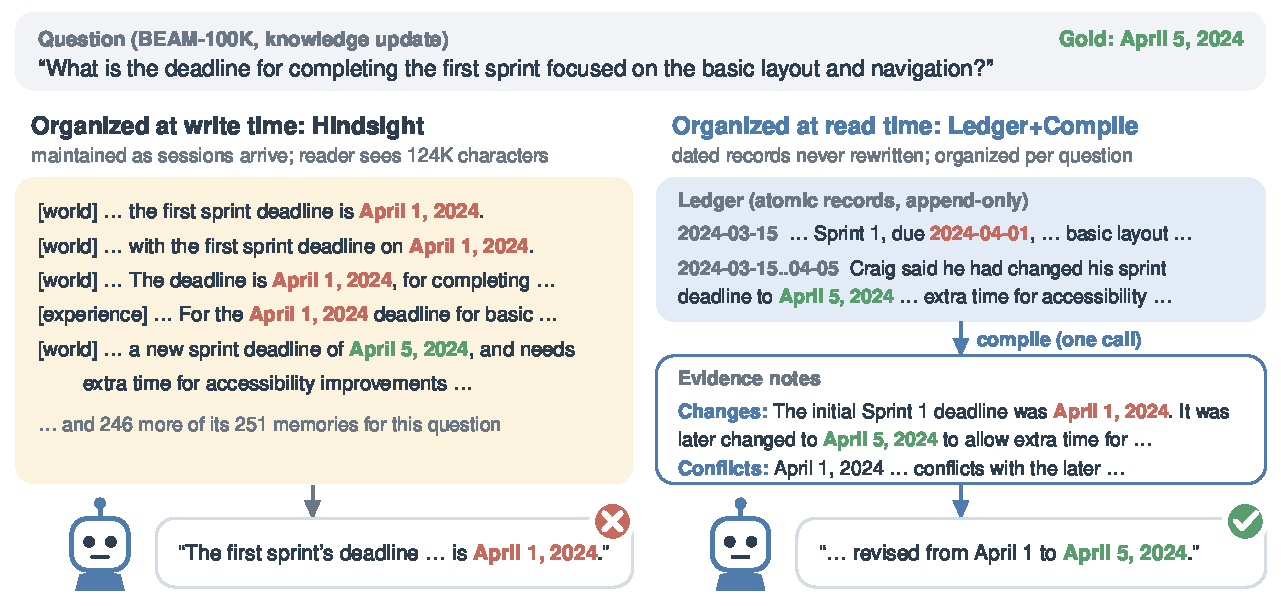
\includegraphics[width=\linewidth]{figs/fig1_teaser.pdf}
\caption{\textbf{The same update, organized at write time and at read time.} A BEAM-100K question whose answer changed
during the conversation. Hindsight's context (left, 251 memories) contains the update, but as one memory among several
that repeat the old date, and the reader gives the old date in all three runs. \method{} keeps both dated records in
its ledger and compiles them for this question into notes that state the change (right); the reader is correct in all
three runs. Quoted text is excerpted from the actual contexts (gpt-6-luna reader, tuned prompt).}
\label{fig:teaser}
\end{figure}

% P3: what we do (A/B round 1: slightly better than ReadAgent's method paragraph; edits applied)
This paper makes that comparison under controlled conditions. We fix a protocol in which only the memory varies:
one reader model, one answer prompt, the official BEAM rubric judge, three independent generations per question, and
confidence intervals clustered by conversation (\cref{sec:setting}). Under this protocol we audit where the scores of
current systems come from, separating the answer prompt, the context budget, and the storage representation
(\cref{sec:audit}). The audit points to the reader as the bottleneck. Of the \prelim{36} points Hindsight loses on
BEAM-1M, \prelim{19.6} come from questions whose answer was already in its context, where the reader did not find
it, did not line up the dates, or did not notice that two statements disagree. Since what a reader needs depends on
the question, we propose to defer organization until the question is known. \method{} (\cref{fig:teaser,fig:overview},
\cref{sec:method}) moves merging, reconciling, and summarizing from write time to read time. The write side only
splits sessions into atomic records and appends them to a ledger that is never rewritten. At question time,
\method{} (1) retrieves a large candidate set of records with hybrid search, (2) compiles them in one call into
question-specific evidence notes (a step we call \emph{compilation}), and (3) gives the reader these notes together with the retrieved records. The
notes order the relevant facts in time and flag updates, conflicts, gaps in coverage, and standing instructions from
the user. We compare against baselines given the same extra call, report the cost of each system, and repeat the main
comparison with three reader models and on LongMemEval~\citep{wu2025longmemeval} (\cref{sec:experiments}).

% P4: findings (A/B round 1: LongMemEval slightly better; round 2 after rewrite: ours slightly better; edits applied)
Our experiments on BEAM at the 100K and 1M tiers and on LongMemEval-S support four findings. Hindsight
always receives an extra read-time call of its own (a conflict check), so no gain below comes from \method{} making
one more call.
\begin{itemize}
\item (\cref{sec:audit}) \textbf{Comparisons at default settings confound storage format with context budget.} On the
100 BEAM-1M development questions, raising Hindsight's budget from 8K to its full 124K characters moves it by
\prelim{25.0} points, while atomic records stay within \prelim{2.1} points at every budget; at equal budgets the format
effect is small and changes sign, from \prelim{$+1.6$} for records at 60K characters to \prelim{$-3.1$} at 124K.
\item (\cref{sec:main,sec:reader}) \textbf{Compiling notes at read time helps, most with a weaker reader.} With
gpt-6-luna as the reader, \method{} leads Hindsight by \prelim{$+7.3$} points on BEAM-100K and \prelim{$+4.2$}
on BEAM-1M (three runs, 95\% intervals above zero). Three stronger readers (DeepSeek-V4.1-Flash, gpt-6.1-sol,
gpt-6-astra) raise Hindsight by \prelim{6} to \prelim{10} points with its memory unchanged, while \method{} gains less;
it stays ahead in all eight reader-and-tier cells, but by only \prelim{1} to \prelim{3} points.
\item (\cref{sec:ablation}) \textbf{Storage format matters once records are compiled into notes.} Notes compiled from
the atomic records that \method{} stores beat the same notes compiled from Hindsight's facts by \prelim{$+6.6$} points on BEAM-100K questions about a single fact or state (95\% interval \prelim{$[+2.6, +11.0]$}), although the
two formats are close when the reader reads them directly (\cref{sec:audit}).
\item (\cref{sec:ablation}) \textbf{Compiled notes are robust to the answer prompt.} The answer prompt that Mem0
published for BEAM adds between \prelim{$+0.7$} and \prelim{$+11.5$} points to systems without notes on BEAM point questions,
but changes the score of compiled notes by at most \prelim{2.3}. On LongMemEval-S the same tuned prompt lowers plain
record retrieval by about \prelim{5} points; with the minimal prompt, \method{} is at or above record retrieval and
Hindsight for all three readers (\cref{tab:lme}).
\end{itemize}

% P5: contributions
In summary, we contribute (i) a controlled protocol and audit that separate the memory from the reader, prompt,
budget, and judge on a 1M-token benchmark; (ii) \method{}, a memory that keeps an append-only ledger and organizes
only at read time, with a compilation format designed for conversational memory; and (iii) evidence across three
readers, two benchmark tiers, and LongMemEval for when read-time organization pays off and when it does not.
\todo{test-set results (BEAM-100K test conversations, BEAM-1M test rows, LongMemEval-S test) once the method is frozen.}

\section{Related Work}
\label{sec:related}

% R1: memory systems (A/B: clearly better than LongMemEval's memory-methods paragraph; positioning fixes applied)
\paragraph{Memory systems for long conversations.}
Memory systems for chat assistants differ in when they organize what they store. MemGPT treats the context window as
virtual memory and lets the agent move and edit content between it and external storage~\citep{packer2023memgpt}.
Most later systems instead store an LLM-processed version of the history and reorganize it at write time, as new turns
or sessions arrive. Mem0 extracts facts and decides for each new fact whether to add it, update an existing one, or
delete one~\citep{chhikara2025mem0}. A-Mem links each new note to related notes and updates the tags and context of
existing ones~\citep{xu2025amem}. MemoryOS moves content between short-, mid-, and long-term
stores~\citep{kang2025memoryos}. Zep builds a temporal knowledge graph whose edges are invalidated rather than deleted
when facts change~\citep{rasmussen2025zep}. Hindsight organizes memory into four networks of world facts, agent
experiences, synthesized entity summaries, and evolving beliefs, and updates them as conversations
arrive~\citep{latimer2025hindsight}. Other systems defer or limit this work: LightMem consolidates long-term memory
offline~\citep{fang2025lightmem}, LycheeMemory encodes each finalized segment of dialogue into context-independent
typed records rather than merging it into existing memory~\citep{li2026lychee}, and LeanMem updates only the event
memories that evolve while keeping source-grounded records unchanged~\citep{liao2026leanmem}. Even these decide what to
merge before any question is asked. A related line handles conflicting memories when they are written: MOSAIC checks
each new fact against its graph neighbors and updates or deletes contradicted entries~\citep{zhao2026mosaic}, TOKI
types contradiction resolution as bitemporal operators~\citep{wang2026toki}, and TEPA revokes stale entries while
keeping them for audit~\citep{zhou2026tepa}. \method{} keeps one write-time step, segment-level extraction of atomic records as
in LycheeMemory, and defers everything that relates records to one another (merging, resolving conflicts, and
summarizing) to read time, where it is conditioned on the question. The price is extra computation for every
question, which we measure in \cref{sec:cost}.

% R2: reading strategies and query-focused compression
\paragraph{Organizing retrieved context for the reader.}
A second line of work organizes text for the reader, either when the index is built or when a query arrives.
RAPTOR recursively clusters and summarizes chunks into a tree that is queried at several levels of
abstraction~\citep{sarthi2024raptor}, and GraphRAG summarizes communities of an entity graph and answers global
questions by map-reduce over these summaries~\citep{edge2024graphrag}; both organize at index time. At query time,
Chain-of-Note trains a model to write a reading note on each retrieved document before answering~\citep{yu2023chainofnote},
RECOMP trains compressors that shorten retrieved documents into extractive or abstractive summaries~\citep{xu2024recomp},
ReadAgent prompts a model to compress pages into gists and look pages up again when needed~\citep{lee2024readagent}, and
Astute RAG consolidates retrieved and internal knowledge and resolves conflicts between them~\citep{wang2024astute}.
Self-RAG~\citep{asai2024selfrag} and Adaptive-RAG~\citep{jeong2024adaptive} decide when and how much to retrieve, which
is complementary to organizing what has been retrieved. Closest to us, LongMemEval finds that Chain-of-Note-style reading
and a structured presentation of retrieved sessions improve accuracy on long chat histories~\citep{wu2025longmemeval}.
Two recent memory systems also move work to query time. Pull keeps raw turns behind a deterministic index and lets the
reader expand only the turns it needs~\citep{chen2026pull}; it does not rewrite what it retrieves. DeferMem is the
closest to our method: it retrieves a broad, noisy candidate set from raw history at query time and distills it into
query-specific evidence with a model trained by reinforcement learning~\citep{yin2026defermem}, evaluated on LoCoMo
and LongMemEval. \method{} differs in three ways: it needs no training, it compiles from extracted records rather
than raw turns and passes the records to the reader along with the notes, and its notes have a fixed structure for
memory-specific failures (updates, conflicts, gaps in coverage, standing instructions). We also evaluate at the 1M
tier of BEAM, where DeferMem has not been tested.
We build on these observations rather than claim reader-side notes as new. Our compilation step is one prompted call per
question, and its format is specific to conversational memory: it orders evidence by time and marks facts that were
later updated or contradicted, parts of the question the memory does not cover, and the user's standing instructions.
Zep tracks the validity of facts at write time; we do so at read time over storage that never changes. Our main
contribution, however, is not the format but a controlled comparison of organizing at write time and at read time,
with retrieval, prompt, and judge held fixed, across readers that differ in how well they use long contexts.

% R3: how readers use long contexts (A/B: clearly better than Lost-in-the-Middle 6.2; edits applied)
\paragraph{How readers use long contexts.}
The \emph{reader}, the model that answers from what the memory retrieves, uses information in the middle of a long
input less reliably than information at its ends~\citep{liu2024lost}, and its effective context is often much shorter
than the window it accepts~\citep{hsieh2024ruler}. These findings suggest that giving the reader more memory context
need not raise accuracy. We observe this in memory systems as well, and we find that it varies sharply across
readers: the long-context gap that our compilation step (\cref{sec:method}) closes for one reader is already small
for another (\cref{sec:reader}).

% R4: evaluating memory systems
\paragraph{Evaluating long-term memory.}
LoCoMo~\citep{maharana2024locomo}, LongMemEval~\citep{wu2025longmemeval}, and BEAM~\citep{tavakoli2025beam} test
memory over conversations ranging from about 9K tokens (LoCoMo) to 10M tokens (BEAM). LongMemEval and BEAM grade
free-form answers with an LLM judge, whose verdicts depend on the judge model and its prompt~\citep{zheng2023judging}.
Numbers reported in different papers therefore differ in reader, answer prompt, context budget, and judge, and are
not directly comparable. RENDER fixes the conversation and varies only the form in which evidence reaches the reader,
and finds spreads of 25--49 points across forms on LongMemEval~\citep{si2026render}; \citet{jiang2026presentation}
find that most of the gain of a fine-grained revision ledger disappears once its presentation is matched by a flat
baseline; and MemConflict separates retrieval from use of retrieved evidence under conflicting
memories~\citep{tao2026memconflict}. Our audit makes the same kind of argument for budget and answer prompt on
BEAM, and adds a split of each system's lost points into storage, retrieval, and reading. We do not propose a new benchmark. Within each comparison we evaluate every system with the
same reader, prompt, and judge, run each condition three times, and report intervals clustered by conversation, so
that for a given reader the differences between rows reflect the memory rather than the evaluation setup; we then
repeat the main comparison with three readers (\cref{sec:setting}).

\section{Setting and Controlled Protocol}
\label{sec:setting}
% A/B round 1: S1-S2 clearly better than LongMemEval 3.1-3.2; S3-S5 comparable to Lost in the Middle 2.1.
% Edits applied: fixed ingestion model, splits with seeds, call-count honesty, judge caveat, prompt numbers, decoding.

% S1: task
\paragraph{Task.}
A conversation is a sequence of dated sessions between a user and an assistant. A memory system reads the sessions in
order and maintains a store, calling an ingestion LLM and an embedding model as it needs. After the last session it
receives a question $q$ and the current date, builds a context $C(q)$ from its store, and a \emph{reader} model answers
$q$ from $C(q)$ under an answer prompt $P$. A judge model grades the answer. The score of a system therefore depends on
the memory through $C(q)$, but also on the reader, on $P$, on the length of $C(q)$, and on the judge. Our protocol
fixes the reader, $P$, and the judge, fixes the ingestion LLM and the embedding model across systems, and reports the
length of $C(q)$ for every system, so that two rows in a table differ in the memory, or in a single named factor
that we vary deliberately.

% S2: data
\paragraph{Data.}
BEAM~\citep{tavakoli2025beam} has 2,000 questions over 100 synthetic conversations in four length tiers. Every
session carries a date, and each conversation contains two questions for each of ten abilities: abstention,
contradiction resolution, event ordering, information extraction, instruction following, knowledge update,
multi-session reasoning, preference following, summarization, and temporal reasoning. We use the 100K tier
(20 conversations) and the 1M tier, where a conversation spans about 1,700 turns and 530,000 words, several times
more than the context we give any reader. We fixed the splits before running any experiment. On BEAM-100K, we
shuffle the 20 conversations with seed 0 and use the first ten (200 questions) for development and the other ten
(200 questions) for testing. On BEAM-1M, the first five conversations in the released order (100 questions) are
for development; of the remaining 30, we fixed the next ten (200 questions) for testing before running any test, because building every memory for all 30 would exceed our budget.
LongMemEval-S~\citep{wu2025longmemeval} gives each of its 500 questions its own history of about 115K tokens. We
stratify questions by type, treating abstention variants as their own stratum, and draw with seed 0 a development set
of \prelim{62} questions and a disjoint test set of 151; the remaining questions are unused. Every result before
\cref{sec:test} comes from development sets, and baselines are configured on the same development sets.

% S3: readers, judge, prompts
\paragraph{Readers, judge, and prompts.}
Our main reader is gpt-6-luna. To test whether conclusions depend on the reader, we repeat the main comparison with
DeepSeek-V4.1-Flash (weights of 2026-10-17, served with vLLM on eight H20 GPUs), with gpt-6.1-sol, and, for one run
because of its cost, with gpt-6-astra. Within a
comparison, every system uses the same reader, and every LLM call it makes at read time (query planning, conflict
checks, compilation) uses that reader too. Memory stores are built once with gpt-6-luna and shared, and Hindsight's
recalled contexts are computed once and reused; swapping the reader therefore tests the read side only. Answers and
compilation use medium reasoning effort; conflict checks and grading use low effort (thinking disabled for
DeepSeek). All answers are graded by gpt-6-luna with each benchmark's official prompt: on BEAM, a rubric prompt that
scores each rubric item 0, 0.5, or 1, averaged per question; on LongMemEval, a yes/no correctness prompt. Because the
judge is also the main reader, we keep it fixed when other models read \todo{re-grade a random subset with
gpt-6.1-sol and report agreement}. We use two answer prompts. The \emph{minimal} prompt tells the reader that
earlier sessions are no longer available, that only its memory of them is shown, and that it should reply as the
assistant using that memory. The \emph{tuned} prompt is the answer
prompt that Mem0 released for BEAM, which tells the reader to scan all memories, cross-check them, and use a fixed
sentence for abstention. On BEAM-1M it raises Hindsight by \prelim{8.6} points but our compiled notes by at most
\prelim{2.3} (\cref{sec:ablation}), so we report BEAM comparisons under the tuned prompt and name the prompt wherever it
changes.

% S4: baselines and budgets
\paragraph{Systems and budgets.}
Our main baseline is Hindsight~\citep{latimer2025hindsight}, which reports the highest BEAM scores among systems with
released code that we could run. We use its server (version 1.0.0) with gpt-6-luna for fact extraction; its recall
returns about 124K characters per question. Hindsight reports \prelim{73.9} on BEAM-1M with its own reader and judge;
under our protocol it scores \prelim{70.4} with the tuned prompt. Because \method{} makes read-time calls besides the
answer, we also run Hindsight\,+\,CC, which adds one call: a conflict check that lists retrieved memories that
disagree with each other and appends them to the context. \method{} still makes one more call than Hindsight\,+\,CC
(query planning, which the record-retrieval baseline also uses); \cref{sec:cost} reports the tokens each system
spends. We further report record retrieval, a re-implementation of LycheeMemory~\citep{li2026lychee} over the same
records that \method{} stores, with its default 8K-character context and, in \cref{sec:audit}, budgets up to 124K
characters; plain retrieval of raw dialogue chunks; and, on BEAM-100K, the full conversation. Embeddings come from
Qwen3-Embedding-8B, and hybrid search fuses dense and BM25 rankings by reciprocal rank. \Cref{tab:systems} lists the
calls and context length of each system.

% S5: statistics
\paragraph{Repetition and statistics.}
Every condition is run three times, with independent generations of every read-time LLM call; the store is built
once. We average the three scores of each question and compare systems on the same questions. Questions within a
conversation are correlated, so we resample whole conversations (5,000 bootstrap draws) and report 95\% percentile
intervals for differences between systems. On the 200 BEAM-100K development questions, the 95\% interval of a
single-generation score spans roughly $\pm$5 points, so we draw conclusions from three-run averages and mark every
single-run result.

\begin{table}[t]
\centering\small
\caption{Systems compared. ``Calls'' are LLM calls; ``ctx'' is the average context, in characters, that the reader
receives on BEAM-1M. $^\dagger$On BEAM-100K, the only tier where the conversation fits. \method{}'s context is the
notes plus the retrieved records. \todo{report tokens as well as characters; Hindsight write-time tokens.}}
\label{tab:systems}
\begin{tabular}{lllr}
\toprule
System & Write-time calls & Read-time calls & ctx \\
\midrule
Full context & none & answer & \prelim{675K}$^\dagger$ \\
Raw-chunk retrieval & none (embeddings) & answer & \prelim{7.4K} \\
Record retrieval (LycheeMemory) & 1 per segment & plan, answer & \prelim{7.6K} \\
Hindsight & fact extraction, entity summaries & answer & \prelim{124K} \\
Hindsight\,+\,CC & same & conflict check, answer & \prelim{124K} \\
\method{} & 1 per segment & plan, compile, answer & \prelim{64K} \\
\bottomrule
\end{tabular}
\end{table}

\section{Where Do Memory Scores Come From?}
\label{sec:audit}
% A/B: 4.1-4.2 passed in round 2, 4.3-4.4 in round 3. 10-17 user request: fewer inline numbers, figures instead of
% tables; intervals moved to the appendix (\cref{app:detail}).

Before proposing a method, we use the protocol of \cref{sec:setting} to measure how much of a memory system's score
comes from the memory and how much from its surroundings. All numbers in this section are on development sets with
gpt-6-luna as reader and judge; intervals for every difference are in \cref{app:detail}. With 100 BEAM-1M or 200
BEAM-100K questions, single-run differences below about 4 points are not resolved.

% A1: prompt
\subsection{The answer prompt shifts scores by several points}
\label{sec:audit-prompt}
\Cref{tab:prompt} keeps every context fixed and changes only the answer prompt. The prompt that Mem0 released for
BEAM raises Hindsight on BEAM-1M by about 9 points in one run (about 5 over three runs) and record retrieval by about
4; on BEAM-100K it helps both memories by about 2 points and lowers the full-context reader by 4. None of the resulting
rank changes is resolved, so we claim only that the answer prompt moves absolute scores by as much as many published
differences between systems, not that it reorders the systems we test. We use the tuned prompt in the rest of the
paper because it is the public answer prompt for BEAM, and neither prompt was adjusted on our development questions.

\begin{table}[t]
\centering\small
\caption{Changing only the answer prompt (one run each, contexts unchanged). Minimal: our plain prompt; tuned: the BEAM
answer prompt released by Mem0; CC: conflict check. Intervals in \cref{app:detail}.}
\label{tab:prompt}
\begin{tabular}{lrrrrrr}
\toprule
& \multicolumn{3}{c}{BEAM-100K} & \multicolumn{3}{c}{BEAM-1M} \\
\cmidrule(lr){2-4}\cmidrule(lr){5-7}
System & minimal & tuned & $\Delta$ & minimal & tuned & $\Delta$ \\
\midrule
Full context & \prelim{69.9} & \prelim{65.9} & \prelim{$-4.0$} & --- & --- & --- \\
Record retrieval\,+\,CC & \prelim{67.5} & \prelim{69.7} & \prelim{$+2.2$} & \prelim{64.6} & \prelim{68.7} & \prelim{$+4.1$} \\
Hindsight & \prelim{66.5} & \prelim{69.1} & \prelim{$+2.6$} & \prelim{63.7} & \prelim{72.3} & \prelim{$+8.6$} \\
\bottomrule
\end{tabular}
\end{table}

\begin{figure}[t]
\centering
\begin{subfigure}[b]{0.47\linewidth}\centering
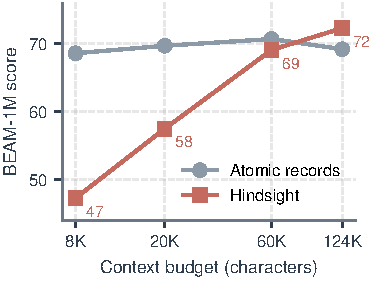
\includegraphics[width=\linewidth]{figs/fig3_budget.pdf}
\caption{Score against context budget.}\label{fig:budget}
\end{subfigure}\hfill
\begin{subfigure}[b]{0.50\linewidth}\centering
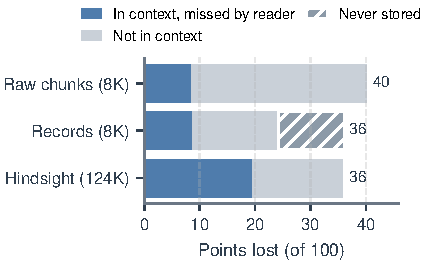
\includegraphics[width=\linewidth]{figs/fig4_loss.pdf}
\caption{Where the lost points go.}\label{fig:loss}
\end{subfigure}
\caption{\textbf{Budget and reader, not storage format, separate the systems on BEAM-1M} (100 development questions,
one run). (a) Atomic records score about the same at every budget; Hindsight needs its full 124K characters. (b) The
8K systems lose most points to information that never reached the reader; Hindsight loses about half of its points to
information that was in its context.}
\label{fig:audit}
\end{figure}

% A2: budget x format
\subsection{Hindsight needs a large context budget; atomic records do not}
\label{sec:audit-budget}
Hindsight stores narrative facts with entity summaries and hands the reader 124K characters; record retrieval stores
atomic records and hands it 8K. \Cref{fig:budget} separates format from budget by cutting each system's ranked
context, at memory boundaries, to the same length. Atomic records stay within about 2 points of each other from 8K to
124K characters. Hindsight falls to 47 at 8K, about 21 points below records, is level with them from 60K on, and is
ahead by 3 points at 124K in this run. The steep curve has a likely mechanical cause: Hindsight's top-ranked memories
carry long raw excerpts, and an 8K cut keeps a median of 2 of its 223 retrieved memories. A comparison of the two
systems at their default settings therefore confounds the format with the budget.

% A3: where the points are lost
\subsection{The 8K systems lose points at retrieval, Hindsight about half at the reader}
\label{sec:audit-loss}
For every rubric item an answer misses, we ask gpt-6-luna whether the information the item needs appears in the
context the reader received and, for record retrieval, whether it appears anywhere in the stored records. A second
judge, gpt-6.1-sol, agrees on 92\% of a 50-item sample for each 8K system and on 76\% for Hindsight, whose long
contexts are harder to check; where they disagree on Hindsight, gpt-6.1-sol more often finds the information in
context, so the reader share below is, if anything, an underestimate. \Cref{fig:loss} shows the split on BEAM-1M. The
two 8K systems lose most of their points before the reader sees anything: raw-chunk retrieval loses 32 of its 40
points to information missing from its context, and record retrieval loses 15 to records that were stored but not
retrieved and 12 to information no record holds. Hindsight's longer context does not lower the total loss (36 points),
but about half of it (20 points) comes from information that was in front of the reader. Because the three systems
differ in more than context length, this describes where they lose points rather than testing whether length causes
reader errors. Raw text is not the remedy either: at a 20K-character budget, replacing each retrieved record with the
dialogue turns it came from lowered BEAM-100K by about 10 points (one run, 120 questions).

% A4: write-time changes
\subsection{The write-time changes we tried did not raise scores}
\label{sec:audit-write}
Before turning to the read side, we tried three changes to what the record store keeps, each on BEAM-100K with record
retrieval as the base. Anchoring each record to verbatim quotes did not change the score over three runs. Keeping both
sides of every contradiction instead of resolving one lowered contradiction questions, because the reader still
ignored the conflict: both statements reached it in 14 of 20 questions, and it raised the conflict in only about half
of those. Keying records by proposition, so that later statements would chain to earlier ones, failed before any
answer was produced, because the two sides of a contradiction never received the same key. Rewriting the store in
place was worse than leaving it alone. In a drift test on LoCoMo, a summary rewritten after every session ended about
20 points below a summary of the same length rebuilt from the untouched ledger, and on BEAM-1M even gpt-6.1-sol, writing
an 8K summary, kept fewer ledger facts when it rewrote than when it rebuilt. \Cref{app:detail} gives counts and tests.
These results do not rule out better write-time designs, but they point to the read side, where \cref{fig:loss} places
about half of the losses of the one system with a long context.

\section{Organizing Memory at Read Time}
\label{sec:method}

\begin{figure}[t]\centering
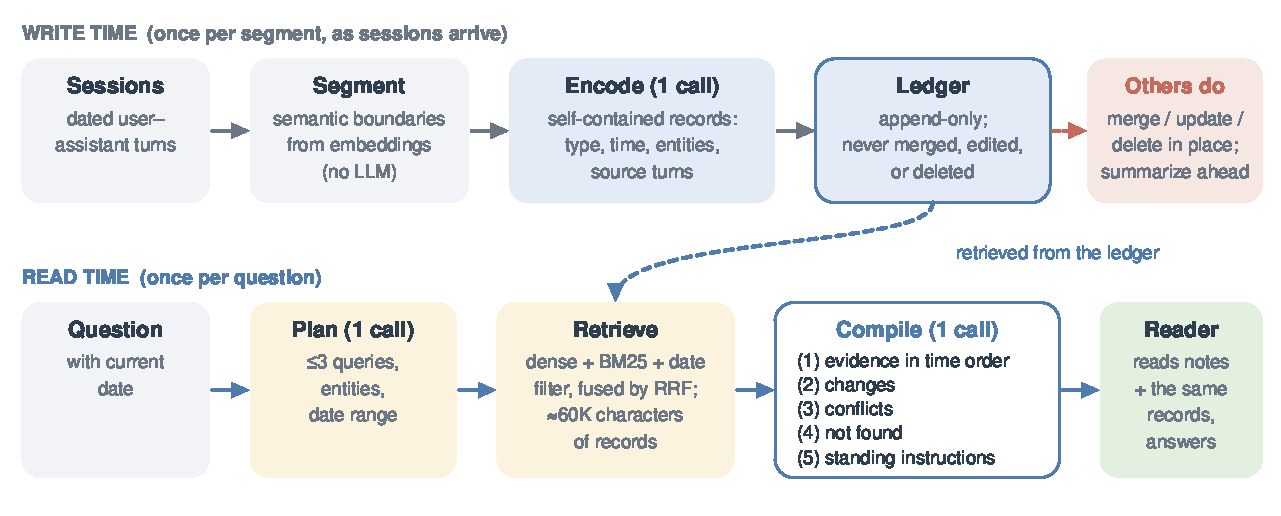
\includegraphics[width=\linewidth]{figs/fig2_method.pdf}
\caption{\textbf{\method{}.} At write time (top), each segment of a session is encoded once into self-contained,
dated records that are appended to a ledger and never merged, edited, or deleted, unlike systems that consolidate
their store in place. At read time (bottom), one call plans the search, hybrid retrieval returns about 60K characters
of records, one call compiles them into five-part evidence notes, and the reader answers from the notes and the same
records.}
\label{fig:overview}
\end{figure}

\Cref{sec:audit} suggests three requirements. The store should keep what was said without rewriting it
(\cref{sec:audit-write}); the reader should receive enough of it that retrieval is not the bottleneck
(\cref{sec:audit-loss}); and the reader should not be left to find, order, and reconcile that material on its own,
which is where Hindsight, the one long-context system in \cref{fig:loss}, loses \prelim{19.6} of its \prelim{36.3} lost points. \method{} meets them with a write side that only
appends, and a read side that retrieves broadly and then organizes what it retrieved for the question at hand
(\cref{fig:overview}). The write side and the retrieval follow LycheeMemory; what is new is the per-question compilation step and giving the reader both the notes and the records.

% M1: write side
\paragraph{Write side: an append-only ledger of atomic records.}
We follow LycheeMemory~\citep{li2026lychee} for the write side. Each session is split into segments at semantic boundaries, placed where adding the next turn would lower a segment's embedding cohesion, without an LLM. One LLM call per
segment turns it into atomic records. Each record is a self-contained statement with resolved names and absolute
dates, a type (event, fact, preference, plan, relation, or opinion), its entities and topic, the time it refers to,
and pointers to the source turns. The call also receives and updates a short disambiguation state (who is who, what
nicknames refer to, which threads are open), which carries context from one segment to the next; the state is a working variable of the encoder and is not part of the stored memory. Records are appended
and never edited, merged, or deleted: a later statement that contradicts an earlier one becomes a new record, and both
remain. A BEAM-1M conversation yields about \prelim{1,350} records.

% M2: retrieval
\paragraph{Step 1: broad retrieval.}
At question time, one short call plans the search: up to three queries, the entities the answer must involve, and a
date range if the question restricts one. Each query is run against the records twice, by dense similarity and by
BM25 over text, entities, and topic, and records inside the date range form one more ranking; reciprocal rank fusion
merges the rankings ($k=60$). We drop a record whose word-level Jaccard overlap with a higher-ranked record exceeds 0.8, attach the source turns of the six best
records, add the eight raw turns that best match the question under BM25, and fill the context up to 60K characters in rank order. This is
LycheeMemory's retrieval with a budget about eight times larger than its default; \cref{sec:audit-budget} shows that
atomic records do not lose accuracy at this budget when read directly, and \cref{sec:ablation} shows that compiling
from it is better than compiling from the default 8K.

% M3: compilation
\paragraph{Step 2: compilation into evidence notes.}
One call receives the question and the retrieved records and writes notes of at most 6,000 characters, without
answering. The notes have five parts:
(1) \emph{evidence}: every relevant item, close to the memory's own words and with its date, in time order and grouped
by thread, with names, numbers, versions, and dates kept exactly;
(2) \emph{changes}: values or plans that changed, from oldest to newest;
(3) \emph{conflicts}: statements that disagree, with both sides;
(4) \emph{not found}: the parts of the question that the memory does not cover; and
(5) \emph{standing instructions}: instructions or preferences the user gave earlier about how answers should be
written or what they should include, quoted with their date, when they could apply to this question.
Each part targets a loss we observed. Evidence in time order serves event ordering, temporal reasoning, and
summarization; changes serve knowledge updates; conflicts serve contradiction questions, where readers saw both sides
and did not raise the conflict (\cref{sec:audit-write}); ``not found'' serves abstention; and standing instructions serve instruction following: on the 10 instruction-following point questions of BEAM-100K, notes without part (5) scored \prelim{62.5}, below record retrieval with a conflict check (\prelim{70.0}), and notes with it \prelim{85.8} (three runs; \cref{sec:ablation}). Removing one part at a time (\cref{tab:noteparts}) lowers the score of the abilities each part targets with gpt-6-luna, by 1 to 2 points overall; ``not found'' has no measurable effect, and with a stronger reader no part matters. The prompt is in \cref{app:prompts}.

% M4: reader
\paragraph{Step 3: the reader reads notes and records.}
The reader receives the notes, followed by the same retrieved records, and answers with the answer prompt shared by all systems in a comparison (\cref{sec:setting}). Keeping the records serves two purposes. The notes are lossy, and the reader can check a detail against
the record it came from. And a reader that uses long contexts well can draw on material that the notes left out,
which matters for the stronger readers in \cref{sec:reader}. An earlier variant that gave the reader the notes and
only 8K characters of records needed a router to send questions about a whole topic to a larger context; giving all
questions the same input removes the router without loss (\cref{sec:ablation}).

% M5: what it costs and what it does not do
\paragraph{Cost and scope.}
At write time, \method{} makes one call per segment, about \prelim{2.3K} input and \prelim{0.8K} output tokens each.
At read time it makes three sequential calls (plan, compile, answer) with the reader model; on BEAM-1M the compilation call reads about \prelim{12K} tokens and the answer call about \prelim{15K}, fewer in total than Hindsight's single answer call over its 124K-character context (\prelim{33K}) and Hindsight\,+\,CC (\prelim{47K}; \cref{sec:cost}). Compilation is repeated for every question, so a system
that answers many questions about the same history pays it many times; caching notes across related questions is
possible but not evaluated here. \method{} does not change what is stored: errors made when a segment is encoded stay
in the ledger, and \prelim{12.0} of the \prelim{36.1} points (out of 100) that record retrieval loses on BEAM-1M come from information that no record holds (\cref{fig:loss}).

\section{Experiments}
\label{sec:experiments}
% 10-17 user request: figures for readers and abilities, fewer inline numbers; per-ability table moved to the appendix.

We compare \method{} with the systems of \cref{tab:systems} under the protocol of \cref{sec:setting}: tuned answer
prompt on BEAM, minimal prompt on LongMemEval, gpt-6-luna as judge, development sets only.

% E1: main results
\subsection{Main results}
\label{sec:main}
\begin{table}[t]
\centering\small
\caption{BEAM development sets, tuned answer prompt, gpt-6-luna judge. Mean of three runs except where
marked. Brackets: \method{} minus Hindsight\,+\,CC, 95\%
interval resampled by conversation, computed from unrounded scores. 200 questions (10 conversations) on BEAM-100K,
100 (5) on BEAM-1M. The tuned prompt is Mem0's public BEAM prompt, not tuned for any system here. $^\ddagger$one run.}
\label{tab:main}
\begin{tabular}{llrr}
\toprule
Reader & System & BEAM-100K & BEAM-1M \\
\midrule
\multirow{6}{*}{gpt-6-luna}
& Full context & \prelim{65.9}$^\ddagger$ & --- \\
& Record retrieval\,+\,CC & \prelim{69.7}$^\ddagger$ & \prelim{68.7}$^\ddagger$ \\
& Hindsight & \prelim{68.2} & \prelim{70.4} \\
& Hindsight\,+\,CC & \prelim{69.5} & \prelim{71.2} \\
& \method{} & \textbf{\prelim{76.8}} & \textbf{\prelim{75.4}} \\
& \quad $\Delta$ vs.\ Hindsight\,+\,CC & \prelim{$+7.3$ $[+4.5, +10.3]$} & \prelim{$+4.2$ $[+1.4, +8.3]$} \\
\midrule
\multirow{4}{*}{DeepSeek-V4.1-Flash}
& Hindsight & \prelim{75.3} & \prelim{75.2} \\
& Hindsight\,+\,CC & \prelim{76.0} & \prelim{76.7} \\
& \method{} & \textbf{\prelim{76.8}} & \textbf{\prelim{79.9}} \\
& \quad $\Delta$ vs.\ Hindsight\,+\,CC & \prelim{$+0.8$ $[-1.1, +2.9]$} & \prelim{$+3.2$ $[-0.6, +5.7]$} \\
\midrule
\multirow{4}{*}{gpt-6.1-sol}
& Hindsight & \prelim{76.8} & \prelim{78.8} \\
& Hindsight\,+\,CC & \prelim{77.0} & \prelim{78.9} \\
& \method{} & \textbf{\prelim{78.9}} & \textbf{\prelim{80.2}} \\
& \quad $\Delta$ vs.\ Hindsight\,+\,CC & \prelim{$+1.9$ $[-0.2, +3.9]$} & \prelim{$+1.3$ $[-3.0, +5.5]$} \\
\midrule
\multirow{4}{*}{gpt-6-astra$^\ddagger$}
& Hindsight & \prelim{75.3} & \prelim{80.4} \\
& Hindsight\,+\,CC & \prelim{76.7} & \prelim{79.5} \\
& \method{} & \textbf{\prelim{79.7}} & \textbf{\prelim{80.9}} \\
& \quad $\Delta$ vs.\ Hindsight\,+\,CC & \prelim{$+2.9$ $[+0.1, +5.6]$} & \prelim{$+1.4$ $[-4.8, +7.0]$} \\
\bottomrule
\end{tabular}
\end{table}

\paragraph{\method{} has the highest score in every cell; the gain is resolved with gpt-6-luna.}
\Cref{tab:main} gives the main comparison. With gpt-6-luna as reader, \method{} leads Hindsight\,+\,CC by 7 points on
BEAM-100K and 4 on BEAM-1M over three runs, and both intervals exclude zero. It also leads the record-retrieval system
that shares its records by about 7 points on both tiers; that system retrieves 8K characters and makes no compilation
call, and \cref{tab:ablation} separates the two factors. With the three stronger readers,
\method{} again has the highest score in all six cells, by about 1 to 3 points over Hindsight\,+\,CC, resolved only for
gpt-6-astra on BEAM-100K (\cref{sec:reader}).

\begin{figure}[t]
\centering
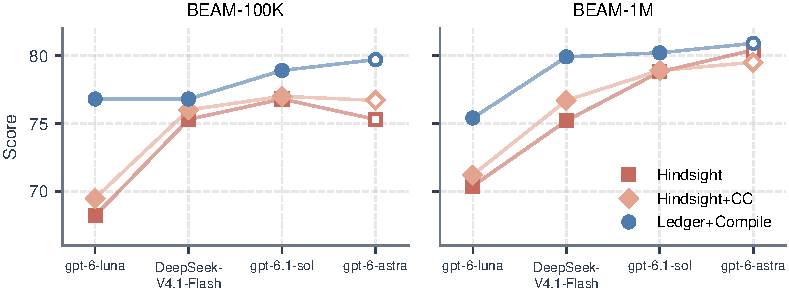
\includegraphics[width=0.98\linewidth]{figs/fig5_readers.pdf}
\caption{\textbf{Stronger readers close the gap.} Scores with four readers and the same memories (tuned prompt,
gpt-6-luna judge). Filled markers: mean of three runs; open markers: one run (gpt-6-astra, because of its
cost). Hindsight gains 6 to 10 points when gpt-6-luna is replaced by a stronger reader; \method{} gains
less, and stays ahead in every cell.}
\label{fig:readers}
\end{figure}

\paragraph{Gains concentrate on updates, instructions, and abstention; summarization is worse.}
\Cref{fig:ability} breaks the gpt-6-luna results down by ability (full table in \cref{app:detail}). Each ability has
only 20 questions on BEAM-100K and 10 on BEAM-1M, so single bars are noisy, but the pattern is consistent across the two
tiers. The largest gains are on knowledge update and instruction following on both tiers and on abstention on BEAM-100K,
followed by temporal reasoning and contradiction resolution, the abilities that the parts of the notes target
(\cref{sec:method}). \method{} is worse on summarization on both tiers, and roughly level on information extraction,
multi-session reasoning, and preference following. Summaries need broad coverage of a topic, which a 6,000-character
note that keeps exact items does not give; raising the limit to 15,000 characters did not help, because the notes
rarely used the extra room (\cref{app:detail}).

\begin{figure}[t]
\centering
\begin{minipage}[t]{0.48\linewidth}\vspace{0pt}\centering
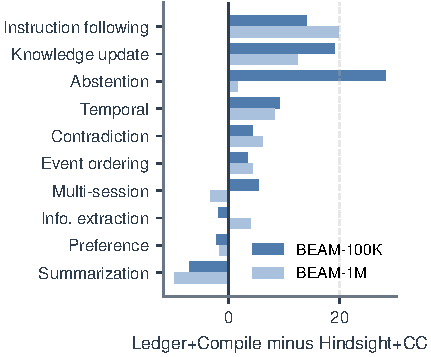
\includegraphics[width=\linewidth]{figs/fig6_ability.pdf}
\end{minipage}\hfill
\begin{minipage}[t]{0.48\linewidth}\vspace{4pt}
\caption{\textbf{Where \method{} gains and loses} (gpt-6-luna, three runs, difference to Hindsight\,+\,CC in points).
Knowledge update, instruction following, and abstention gain the most; summarization loses on both tiers. Each bar
covers 20 (BEAM-100K) or 10 (BEAM-1M) questions.}
\label{fig:ability}
\end{minipage}
\end{figure}

\paragraph{LongMemEval-S.}
We repeat the comparison on the 62 LongMemEval-S development questions with the minimal prompt, the same three
readers, and a Hindsight store built for each question's history (\cref{tab:lme}). \method{} is never below either
baseline. Its lead over Hindsight is largest with gpt-6-luna and smallest with gpt-6.1-sol, the same ordering as on
BEAM. One failure of Hindsight does not depend on the reader: on questions about what the assistant said earlier, it
answers about half correctly with every reader, while both record-based systems answer all of them, because its
extraction keeps mainly facts about the user. Most other questions are answered correctly by every system, so the
remaining differences are within the noise of 62 questions. \todo{test set.}

\begin{table}[t]
\centering
\small
\caption{LongMemEval-S development set (62 questions, minimal prompt, mean of three runs, gpt-6-luna judge).
Differences are \method{} minus the baseline, with 95\% paired bootstrap intervals over questions.}
\label{tab:lme}
\setlength{\tabcolsep}{4pt}
\resizebox{\linewidth}{!}{%
\begin{tabular}{lccccc}
\toprule
Reader & \method{} & Records (8K) & Hindsight & vs.\ records & vs.\ Hindsight \\
\midrule
gpt-6-luna & \prelim{84.4} & \prelim{82.3} & \prelim{71.0} & \prelim{$+2.2$} {\scriptsize[$-5.4$, $+10.8$]} & \prelim{$+13.4$} {\scriptsize[$+3.8$, $+23.1$]} \\
DeepSeek-V4.1-Flash & \prelim{93.5} & \prelim{86.6} & \prelim{85.5} & \prelim{$+7.0$} {\scriptsize[$+1.1$, $+13.4$]} & \prelim{$+8.1$} {\scriptsize[$+0.5$, $+16.1$]} \\
gpt-6.1-sol & \prelim{89.8} & \prelim{89.8} & \prelim{86.0} & \prelim{$+0.0$} {\scriptsize[$-4.8$, $+4.8$]} & \prelim{$+3.8$} {\scriptsize[$-6.5$, $+14.5$]} \\
\bottomrule
\end{tabular}}
\end{table}

% E2: reader strength
\subsection{What a stronger reader changes}
\label{sec:reader}
Changing the reader while keeping every memory fixed separates what the memory stores from how well the reader uses
it (\cref{fig:readers}). With the same 124K-character context, Hindsight\,+\,CC gains 6 to 10 points when gpt-6-luna
is replaced by DeepSeek-V4.1-Flash, gpt-6.1-sol, or gpt-6-astra, while \method{} gains at most about 5. \method{} stays
ahead in all eight reader-and-tier cells, but with the three stronger readers its lead over Hindsight\,+\,CC is 1 to 3
points and resolved only once (gpt-6-astra on BEAM-100K, one run). The stronger readers recover much of what Hindsight's long context
already contains, which is the reader loss of \cref{fig:loss}; compilation does that work in advance for a weaker
reader. On questions that need many facts at once, the strongest readers already do slightly better with Hindsight's
full context than with \method{}. The two are partly redundant, so \method{} helps most where the reader is weakest.
Intervals for every reader are in \cref{app:detail}.

% E3: ablations
\subsection{Ablations}
\label{sec:ablation}
\begin{table}[t]
\centering\small
\caption{Ablations with gpt-6-luna, tuned prompt, on questions about a single fact or state (point questions: 63 on
BEAM-1M, 128 on BEAM-100K). One run unless marked $^\star$ (three runs). The rows above the line use notes followed by
8K characters of records, the variant on which the components were developed.}
\label{tab:ablation}
\begin{tabular}{lrr}
\toprule
Variant & BEAM-100K & BEAM-1M \\
\midrule
Records only, 8K, + conflict check$^\star$ & \prelim{74.5} & \prelim{76.3} \\
Records only, 60K & --- & \prelim{74.3} \\
Notes from 60K + records 8K (full)$^\star$ & \prelim{81.6} & \prelim{80.7} \\
\quad without standing instructions$^\star$ & \prelim{77.9} & \prelim{79.1} \\
\quad notes only (reader sees $\approx$2K characters) & \prelim{79.6} & \prelim{78.2} \\
\quad notes compiled from 8K instead of 60K & \prelim{76.4} & \prelim{79.4} \\
\quad notes compiled from Hindsight's context$^\star$ & \prelim{75.0} & \prelim{77.6} \\
\midrule
Notes from 60K + records 60K (\method{})$^\star$ & \prelim{81.0} & \prelim{82.5} \\
\bottomrule
\end{tabular}
\end{table}

\paragraph{Compiling, not retrieving more, is the main effect.}
\Cref{tab:ablation} removes one component at a time on point questions. With the same 60K characters of records, the
reader scores about 6 points higher on BEAM-1M when it reads notes compiled from them than when it reads them directly,
so the gain does not come from retrieving more. Retrieving deeply before compiling matters more on BEAM-100K (about 6
points over compiling from 8K) than on BEAM-1M (about 1). Keeping records next to the notes adds 2 to 3 points, and the
standing-instruction part adds about 4 points on BEAM-100K over three runs, almost all of it on instruction following.

\paragraph{Each part of the notes helps the questions it targets.}
\Cref{tab:noteparts} removes one part of the notes at a time from the full method, on all 300 development questions
of both tiers. With gpt-6-luna, removing any part except ``not found'' lowers the score, but by only 1 to 2 points
overall, and only the standing instructions are resolved on their own. The effect of each part is concentrated on the
abilities it was written for: without standing instructions, instruction following drops by about 7 points; without
changes, knowledge update drops by about 6; and abstention drops whichever part is removed, because the structure
helps the reader decide whether the memory covers the question at all. The ``not found'' part has no measurable effect
and could be dropped. With gpt-6.1-sol no part has a resolved effect, and removing the standing instructions, if anything, helps
(one run on BEAM-100K: $+2.6$): a strong reader finds and follows earlier instructions in the records itself, while a weaker reader needs
them extracted. Single-run effects were about twice as large as three-run effects for gpt-6-luna, so we report three
runs where we have them.

\begin{table}[t]
\centering\small
\caption{Removing one part of the notes from \method{} (all 300 development questions of BEAM-100K and BEAM-1M,
tuned prompt, gpt-6-luna judge). Differences to the full notes, with 95\% intervals from a bootstrap over
conversations. gpt-6-luna: three runs; gpt-6.1-sol: two runs.}
\label{tab:noteparts}
\begin{tabular}{lcc}
\toprule
Variant & gpt-6-luna & gpt-6.1-sol \\
\midrule
Full notes (score) & \prelim{76.3} & \prelim{78.4} \\
\quad without standing instructions & \prelim{$-1.7$} {\scriptsize[$-3.1$, $-0.4$]} & \prelim{$+0.9$} {\scriptsize[$-0.3$, $+2.1$]} \\
\quad without changes & \prelim{$-1.3$} {\scriptsize[$-2.7$, $+0.2$]} & \prelim{$-0.0$} {\scriptsize[$-1.7$, $+1.6$]} \\
\quad without conflicts & \prelim{$-0.5$} {\scriptsize[$-1.7$, $+0.6$]} & \prelim{$+1.0$} {\scriptsize[$-0.3$, $+2.1$]} \\
\quad without not-found & \prelim{$+0.6$} {\scriptsize[$-1.2$, $+2.3$]} & \prelim{$-0.2$} {\scriptsize[$-1.9$, $+1.7$]} \\
\quad evidence only & \prelim{$-1.7$} {\scriptsize[$-3.5$, $+0.0$]} & \prelim{$+0.1$} {\scriptsize[$-1.8$, $+1.8$]} \\
\bottomrule
\end{tabular}
\end{table}
\todo{one run with DeepSeek-V4.1-Flash (running).}

\paragraph{Compiling from atomic records beats compiling from Hindsight's context.}
The same notes compiled from Hindsight's context instead of from atomic records lose about 7 points on BEAM-100K point
questions (resolved over three runs) and 3 on BEAM-1M (not resolved). The two sources also differ in length, 60K
characters of records against Hindsight's full 124K, so this compares two complete memories rather than two formats at
equal length. Notes still help Hindsight, by about 7 and 4 points over its own context, so compilation also works as a
plug-in. The gap is largest on abstention and knowledge update, where notes compiled from dated, self-contained records
can state when something changed and what was never said. Read directly, the two formats were close at equal budgets
(\cref{fig:budget}); the format starts to matter once something organizes it for the reader.

\paragraph{One input for all questions.}
Before arriving at \method{}, we routed questions about a whole topic to 60K characters of records and gave other
questions notes with 8K characters of records. Giving every question the notes with all 60K characters matches the
routed system over three runs on both tiers and removes the router; with DeepSeek-V4.1-Flash it is about 2 points
ahead on both tiers in one run.

\paragraph{On BEAM-1M, compiled notes are less sensitive to the answer prompt.}
On BEAM-1M point questions, switching from the minimal to the tuned prompt changes compiled notes by less than 1 point,
against about 5 for record retrieval with a conflict check and about 12 for Hindsight (one run each, on the
notes-plus-8K variant); on BEAM-100K all three change by at most about 2 points. On LongMemEval-S, where the tuned prompt was
not written for the benchmark, it lowers record retrieval by about 5 points, and notes with the minimal prompt score
highest. Compilation appears to do part of what the tuned prompt asks the reader to do, scanning everything and
cross-checking. \todo{repeat with \method{} and three runs.}

% E4: cost
\subsection{Cost}
\label{sec:cost}
\Cref{tab:cost} lists read-time tokens per question on BEAM-1M with gpt-6-luna. \method{} reads about 27K input tokens
over three calls, fewer than Hindsight's single answer call over its 124K-character context (33K) and fewer than
Hindsight\,+\,CC (47K); it writes more output tokens (1.5K against 0.4K and 0.2K), mostly the notes. The three calls
are sequential, so latency is roughly that of three model calls. At write time, \method{} makes one call per segment of
about 2K input and 1K output tokens. \todo{segments per conversation; Hindsight's write-time tokens.}

\begin{table}[t]
\centering\small
\caption{Average tokens per question at read time on BEAM-1M (gpt-6-luna; input / output, output includes reasoning; totals from unrounded values).}
\label{tab:cost}
\begin{tabular}{lrrrr}
\toprule
System & Plan & Conflict check / compile & Answer & Total \\
\midrule
Hindsight & --- & --- & \prelim{33.2K / 0.4K} & \prelim{33.2K / 0.4K} \\
Hindsight\,+\,CC & --- & \prelim{13.4K / 0.1K} & \prelim{33.7K / 0.2K} & \prelim{47.1K / 0.2K} \\
\method{} & \prelim{0.1K / 0.1K} & \prelim{12.4K / 1.0K} & \prelim{14.7K / 0.4K} & \prelim{27.2K / 1.5K} \\
\bottomrule
\end{tabular}
\end{table}

% E5: test sets
\subsection{Held-out test sets}
\label{sec:test}
We ran the test sets once, after freezing \method{}, its prompts and the baselines' configurations: the 10
BEAM-100K conversations not used for development (200 questions), BEAM-1M conversations 6--15 (200 questions), and
the 151 LongMemEval-S test questions. Readers, judge, prompts and intervals are those of \cref{tab:main}; on
LongMemEval-S the interval is resampled by question.

\begin{table}[t]
\centering\small
\caption{Held-out test sets, gpt-6-luna reader and judge, mean of three runs. Brackets: \method{} minus the
system in that row, 95\% interval (BEAM: resampled by conversation; LongMemEval-S: by question). Point / aggregate:
questions routed to each answer path (\cref{sec:method}); Hindsight\,+\,CC equals Hindsight on aggregate questions.}
\label{tab:test}
\begin{tabular}{lrrr}
\toprule
System & BEAM-100K & BEAM-1M & LongMemEval-S \\
\midrule
LycheeMemory & --- & --- & \prelim{83.2} \\
Hindsight & \prelim{64.9} & \prelim{61.5} & \prelim{78.6} \\
Hindsight\,+\,CC & \prelim{67.6} & \prelim{64.4} & --- \\
\method{} & \textbf{\prelim{73.7}} & \textbf{\prelim{71.2}} & \textbf{\prelim{85.0}} \\
\midrule
$\Delta$ vs.\ Hindsight & \prelim{$+8.8$ $[+3.7, +13.9]$} & \prelim{$+9.6$ $[+6.4, +12.8]$} & \prelim{$+6.4$ $[+0.9, +11.9]$} \\
$\Delta$ vs.\ Hindsight\,+\,CC & \prelim{$+6.1$ $[+1.1, +10.7]$} & \prelim{$+6.8$ $[+3.4, +10.2]$} & --- \\
$\Delta$ vs.\ LycheeMemory & --- & --- & \prelim{$+1.8$ $[-2.4, +6.0]$} \\
\midrule
Point questions (ours / H+CC / H) & \prelim{76.8 / 67.6 / 63.4} & \prelim{70.2 / 56.8 / 52.0} & --- \\
Aggregate questions (ours / H) & \prelim{67.9 / 67.6} & \prelim{72.6 / 75.3} & --- \\
\bottomrule
\end{tabular}
\end{table}

\paragraph{The development-set gains hold on the test sets.}
\Cref{tab:test} repeats the main comparison on data not used for any decision. On both BEAM tiers \method{} leads
Hindsight\,+\,CC by 6 to 7 points with intervals that exclude zero, as on the development sets (7.3 and 4.2). The
lead comes from questions routed to the point path, where it is 9 to 13 points; on aggregate questions \method{} ties
Hindsight on BEAM-100K and trails it by 2.7 points on BEAM-1M, matching its weakness on summarization
(\cref{sec:limits}). On LongMemEval-S \method{} leads Hindsight by 6.4 points (interval excludes zero) and
LycheeMemory by 1.8 (it does not), the same pattern as on the development set. Every system scores lower on the test
conversations than on the development ones (by 2 to 9 points), most of all Hindsight on BEAM-1M, so the gain does not
shrink on harder data. While building records for LongMemEval-S, the provider's content filter blocked the encoding
output for two segments; those segments contribute no records, and all questions are kept.
\todo{Stronger reader (gpt-6.1-sol) on the test sets.}

\section{Limitations}
\label{sec:limits}
We developed the compilation prompt on the development sets; the held-out test sets (\cref{sec:test}) were run once,
with gpt-6-luna only, and the baselines did not receive a comparable prompt search. gpt-6-luna is the
judge for every reader and also built every memory store, and it is the reader on which our only resolved gains appear,
so a preference of the judge for answers in its own style could inflate them; we have not yet measured agreement with
a second judge or with people. With three stronger readers our gains are small and mostly not resolved. The
development sets are small (200 questions in 10 conversations on BEAM-100K, 100 in 5 on BEAM-1M, 62 on
LongMemEval-S), BEAM conversations are synthetic, and LongMemEval-S is close to its ceiling for the systems we test. We
compare against one strong external system, Hindsight, and our re-implementation of LycheeMemory; other write-time
designs (Mem0, A-Mem, Zep) were not run under the same protocol, and we did not test hybrids that organize at both
write and read time. \method{} makes a compilation call for every question, which adds a second sequential call before the answer; it keeps every encoding error in the ledger; and it is weakest on summarization. The diagnoses in
\cref{sec:audit} rely on an LLM to decide whether information is present in a context; we checked them
against a second LLM but not against people.

\section{Conclusion}
\label{sec:conclusion}
We asked whether a long-term conversational memory should be organized when it is written or when it is read. On BEAM,
under a protocol that fixes the reader, the answer prompt, and the judge, the answer prompt alone (up to \prelim{8.5}
points) and the context budget (up to \prelim{21}) open gaps as large as those between systems, and the one
long-context baseline loses more points to evidence its reader fails to use than to evidence its retrieval fails to
find. Keeping the stored records unchanged and organizing them per question, as \method{} does, outperformed the
write-time system we compared against with gpt-6-luna as reader (\prelim{$+7.3$} and \prelim{$+4.2$} points, three runs);
with three stronger readers it was ahead by 1--3 points in every case, a gap resolved only once. These
results are on development sets and use gpt-6-luna as judge. Two observations may matter beyond our method. The
storage format matters more once something organizes it for the reader: notes compiled from atomic records beat
notes compiled from Hindsight's context by \prelim{6.6} points on BEAM-100K point questions, although the two formats
are close when read directly. And across our three readers, the benefit of read-time organization shrank as the reader used long contexts better, suggesting that how much a memory should organize depends on its reader; confirming this on held-out sets and with a second judge is the main open step.

\bibliography{refs}
\bibliographystyle{iclr2027_conference}
\appendix
\section{Prompts}\label{app:prompts}
\paragraph{Minimal answer prompt (system message).}
{\footnotesize\begin{verbatim}
You are the AI assistant in a long conversation with a user that
spans several sessions. The earlier sessions are no longer available;
only your memory of them is shown below. Reply to the user's new
message as the assistant, using the memory for anything about the
user, their projects, what was said and when, their preferences and
standing instructions.
\end{verbatim}}

\paragraph{Tuned answer prompt (released by Mem0 for BEAM).}
{\footnotesize\begin{verbatim}
You are an AI assistant with access to stored memories from prior
conversations with a user. Use these memories to answer the following
question as accurately and completely as possible.
IMPORTANT RULES:
1. Scan ALL provided memories before answering -- do not stop after
the first relevant one.
2. If multiple memories contain relevant information, combine and
cross-reference them.
3. The question may refer to something indirectly (e.g. 'the person I
met at the festival') -- resolve such references by searching the
memories before concluding. Only if the specific information is
genuinely absent after a careful search, say exactly: "I don't have
enough information to answer this question."
4. Be specific and direct -- include exact names, dates, numbers, and
details from the memories.
5. Do NOT invent or assume information that isn't in the memories.
QUESTION: {query}
RETRIEVED MEMORIES:
{context}
ANSWER:
\end{verbatim}}

\paragraph{Conflict check (Hindsight\,+\,CC and record retrieval\,+\,CC).}
{\footnotesize\begin{verbatim}
You check a memory before it is shown to someone who will answer a
question. You get the question and the memory lines. Find pairs of
lines that state things about the same matter that cannot both be
true (e.g. 'has never done X' vs 'did X'). Do not count a later
update of a plan, value or status as a conflict when the lines show
it changed over time. Output one JSON object, nothing else:
{"conflicts": [{"a": "short quote of one line", "b": "short quote of
the other", "about": "what they disagree on"}]} with an empty list
when there are none.
\end{verbatim}}

\paragraph{Compilation prompt, parts (1)--(4).}
{\footnotesize\begin{verbatim}
You prepare evidence notes for someone who will answer a user's
question from a long memory of past conversations with that user. You
get the question and the memory. Do not answer the question. Write
notes of at most 6000 characters with these parts: (1) Evidence:
every memory item relevant to the question, stated closely to the
memory's own words with its date, in time order, grouped by thread or
topic; keep names, numbers, versions and dates exactly. (2) Changes:
values or plans that changed over time, oldest to newest. (3)
Conflicts: statements that disagree with each other, both sides. (4)
Not found: parts of the question the memory does not cover.
\end{verbatim}}

\paragraph{Compilation prompt, part (5), appended to the above.}
{\footnotesize\begin{verbatim}
(5) Standing instructions: any instruction or preference the user
gave earlier about how answers should be written or what they should
include (format, level of detail, items to always mention), quoted
exactly with its date, when it could apply to an answer to this
question.
\end{verbatim}}

\section{Detailed results}\label{app:detail}
\paragraph{Intervals for \cref{sec:audit}.} One run each, 95\% intervals resampled by conversation. Tuned minus minimal
prompt (\cref{tab:prompt}): BEAM-100K full context $-4.0$ $[-9.4, +1.3]$, record retrieval\,+\,CC $+2.2$
$[-2.3, +7.0]$, Hindsight $+2.6$ $[+0.2, +5.2]$; BEAM-1M record retrieval\,+\,CC $+4.1$ $[+0.9, +6.7]$, Hindsight $+8.6$
$[+3.5, +13.8]$; over three runs, Hindsight on BEAM-1M $+4.6$. Records minus Hindsight at equal budget on BEAM-1M
(\cref{fig:budget}): 8K $+21.3$ $[+12.0, +29.3]$, 20K $+12.2$ $[+4.2, +21.9]$, 60K $+1.6$ $[-3.1, +6.5]$, 124K $-3.1$
$[-5.5, -0.2]$. Loss attribution (\cref{fig:loss}), points out of 100: raw chunks 40.4 (8.6 in context), record
retrieval 36.1 (8.8 in context, 15.4 not retrieved, 12.0 not stored), Hindsight 36.3 (19.6 in context). Judge
agreement on 50 sampled lost items per system: 92\% ($\kappa$ 0.62), 92\% ($\kappa$ 0.79), 76\% ($\kappa$ 0.52).

\paragraph{Readers (\cref{fig:readers}).} \Cref{tab:readers-ci} lists every reader with 95\% intervals resampled by
conversation.

\begin{table}[h]
\centering\small
\caption{\method{} minus Hindsight\,+\,CC and minus Hindsight on the development sets, per reader (tuned prompt,
gpt-6-luna judge, mean over the runs shown).}
\label{tab:readers-ci}
\setlength{\tabcolsep}{4pt}
\resizebox{\linewidth}{!}{%
\begin{tabular}{lccccc}
\toprule
Reader & Runs & \multicolumn{2}{c}{BEAM-100K} & \multicolumn{2}{c}{BEAM-1M} \\
 & & vs.\ HS\,+\,CC & vs.\ HS & vs.\ HS\,+\,CC & vs.\ HS \\
\midrule
gpt-6-luna & 3 & \prelim{$+7.3$} {\scriptsize[$+4.5$, $+10.3$]} & \prelim{$+8.6$} {\scriptsize[$+5.9$, $+11.5$]} & \prelim{$+4.2$} {\scriptsize[$+1.4$, $+8.3$]} & \prelim{$+5.0$} {\scriptsize[$+2.1$, $+8.9$]} \\
DeepSeek-V4.1-Flash & 3 & \prelim{$+0.8$} {\scriptsize[$-1.1$, $+2.9$]} & \prelim{$+1.5$} {\scriptsize[$-0.3$, $+3.7$]} & \prelim{$+3.2$} {\scriptsize[$-0.6$, $+5.7$]} & \prelim{$+4.6$} {\scriptsize[$+2.2$, $+7.0$]} \\
gpt-6.1-sol & 3 & \prelim{$+1.9$} {\scriptsize[$-0.2$, $+3.9$]} & \prelim{$+2.1$} {\scriptsize[$+0.1$, $+3.9$]} & \prelim{$+1.3$} {\scriptsize[$-3.0$, $+5.5$]} & \prelim{$+1.4$} {\scriptsize[$-2.6$, $+5.2$]} \\
gpt-6-astra & 1 & \prelim{$+2.9$} {\scriptsize[$+0.1$, $+5.6$]} & \prelim{$+4.3$} {\scriptsize[$+1.4$, $+7.2$]} & \prelim{$+1.4$} {\scriptsize[$-4.8$, $+7.0$]} & \prelim{$+0.5$} {\scriptsize[$-4.9$, $+6.5$]} \\
\bottomrule
\end{tabular}}
\end{table}

\paragraph{Write-time changes (\cref{sec:audit-write}).} Verbatim anchoring: $+0.3$ over three runs (BEAM-100K). Keeping
both sides of contradictions: $-9.4$ on the 20 contradiction questions (one run). Proposition keys: 0 of 12 annotated
contradictions received a shared key. Returning raw turns instead of records at 20K characters: $-9.7$ on 120 questions
(one run, sign test over questions $p=0.004$). Drift on LoCoMo (6 conversations, 12 questions each): rewritten 52.8,
rebuilt 73.6 (sign test over 72 questions, $p=0.004$). Drift on BEAM-1M with gpt-6.1-sol, 8K budget: rebuilt 72 and
rewritten 48 of 300 ledger probes correct (47 vs.\ 23 discordant, $p=0.006$); the probes favor the rebuilt summary.
All sign tests treat questions as independent and therefore overstate the evidence.

\paragraph{Larger notes.} Raising the note limit from 6,000 to 15,000 characters on questions about a whole topic
(BEAM-1M, one run): 61.9 vs.\ 60.6 overall and 49.9 vs.\ 49.5 on summarization; notes grew from 15.0K to 17.9K
characters of reader context.

\begin{table}[h]
\centering\small
\caption{Per-ability scores with gpt-6-luna (three runs, tuned prompt). HS\,+\,CC: Hindsight with conflict check.}
\label{tab:ability}
\begin{tabular}{lrrrr}
\toprule
& \multicolumn{2}{c}{BEAM-100K} & \multicolumn{2}{c}{BEAM-1M} \\
\cmidrule(lr){2-3}\cmidrule(lr){4-5}
Ability & HS\,+\,CC & \method{} & HS\,+\,CC & \method{} \\
\midrule
Abstention & \prelim{40.0} & \prelim{68.3} & \prelim{55.8} & \prelim{57.5} \\
Contradiction resolution & \prelim{70.0} & \prelim{74.4} & \prelim{62.1} & \prelim{68.3} \\
Event ordering & \prelim{60.2} & \prelim{63.6} & \prelim{41.4} & \prelim{45.8} \\
Information extraction & \prelim{87.7} & \prelim{85.8} & \prelim{82.7} & \prelim{86.7} \\
Instruction following & \prelim{71.7} & \prelim{85.8} & \prelim{71.9} & \prelim{91.7} \\
Knowledge update & \prelim{59.2} & \prelim{78.3} & \prelim{86.7} & \prelim{99.2} \\
Multi-session reasoning & \prelim{77.1} & \prelim{82.5} & \prelim{78.9} & \prelim{75.7} \\
Preference following & \prelim{95.4} & \prelim{93.3} & \prelim{90.0} & \prelim{88.3} \\
Summarization & \prelim{63.2} & \prelim{56.1} & \prelim{62.8} & \prelim{53.0} \\
Temporal reasoning & \prelim{70.4} & \prelim{79.6} & \prelim{80.0} & \prelim{88.3} \\
\bottomrule
\end{tabular}
\end{table}

\end{document}
